\chapter{Inspirace řešení}
\label{chap:2}
Virtuální sdílená tabule je natolik užitečný nástroj, že je na internetu již spousta různých variant řešení.
Odlišit se tedy není snadné, a proto je práce inspirována několika již existujícími weby, které v rámci funkcí rozšiřuje o určité nové nápady.




\section{Analýza vybraných webů}
\label{sec:2.1}
Weby použité pro inspiraci bylo nejdříve potřeba analyzovat jak z hlediska uživatelských nástrojů a rozhraní, tak z hlediska použitých technologií pro dosažení výsledné funkčnosti.
K identifikaci použitých technologií bylo využito standardně zabudovaných vývojářských nástrojů webového prohlížeče, konkrétně v tomto případě prohlížeče Mozilla Firefox ve verzi 86.
Pro inspiraci bylo vybráno celkově pět webů, které jsou níže vypsány od nejméně po nejvíce autorově subjektivně vnímané ideální řešení nástroje pro sdílení virtuální tabule.




\section{Inspirace vybranými weby}
\subsection{Inspirace - classroomscreen.com}
\label{sec:2.2}
Jako první proběhla analýza webu \underline{classroomscreen.com}.
Tato stránka již na první pohled vypadá spíše jako sdílená obrazovka než jako sdílená tabule, což ostatně napovídá i její název.
Obrazovka zobrazuje simulaci jednotlivých oken, které slouží jako kalendář, stopky, generátor hodu kostkou a další.
Jednotlivé okna mají velmi odlišnou funkčnost a působí tedy podobným dojmem jako počítačové aplikace, což umožňuje tento web využít pro velmi různorodé účely.
Rozhraní obsahuje několik základních tlačítek nástrojů pro vytvoření již zmíněných instancí oken.
Na pozadí je od prvního spuštění vykreslen náhodný obrázek většinou s motivem přírody či nějaké kulturní památky, který je možné kdykoliv změnit v nastavení.
Web má jasně vymezené okraje použitelné části plochy, které jsou dané velikostí uživatelova okna prohlížeče.
Není tedy možné se pohybovat libovolně mimo viditelnou oblast.
Web není určen pro spolupráci více uživatelů a je tedy vhodný především pro menší projekty či prezentace.
Jedinou technologií, která stojí za zmínku je zde Canvas API, která je použita k vykreslování grafického výstupu.
\begin{sloppypar*}
Inspirací k bakalářské práci byl tento web pouze díky nástroje pro úpravu poznámek.
Poznámka v bakalářské práci je stejně jako na tomto webu tvořena pomocí Canvasu překrytého HTML elementem \texttt{<div>} využívajícím atribut \texttt{contenteditable="true"}, který umožňuje úpravu vnitřního textu a díky čemuž tato poznámka působí celistvým dojmem.
\end{sloppypar*}
\begin{figure}[h!]
	\centering
	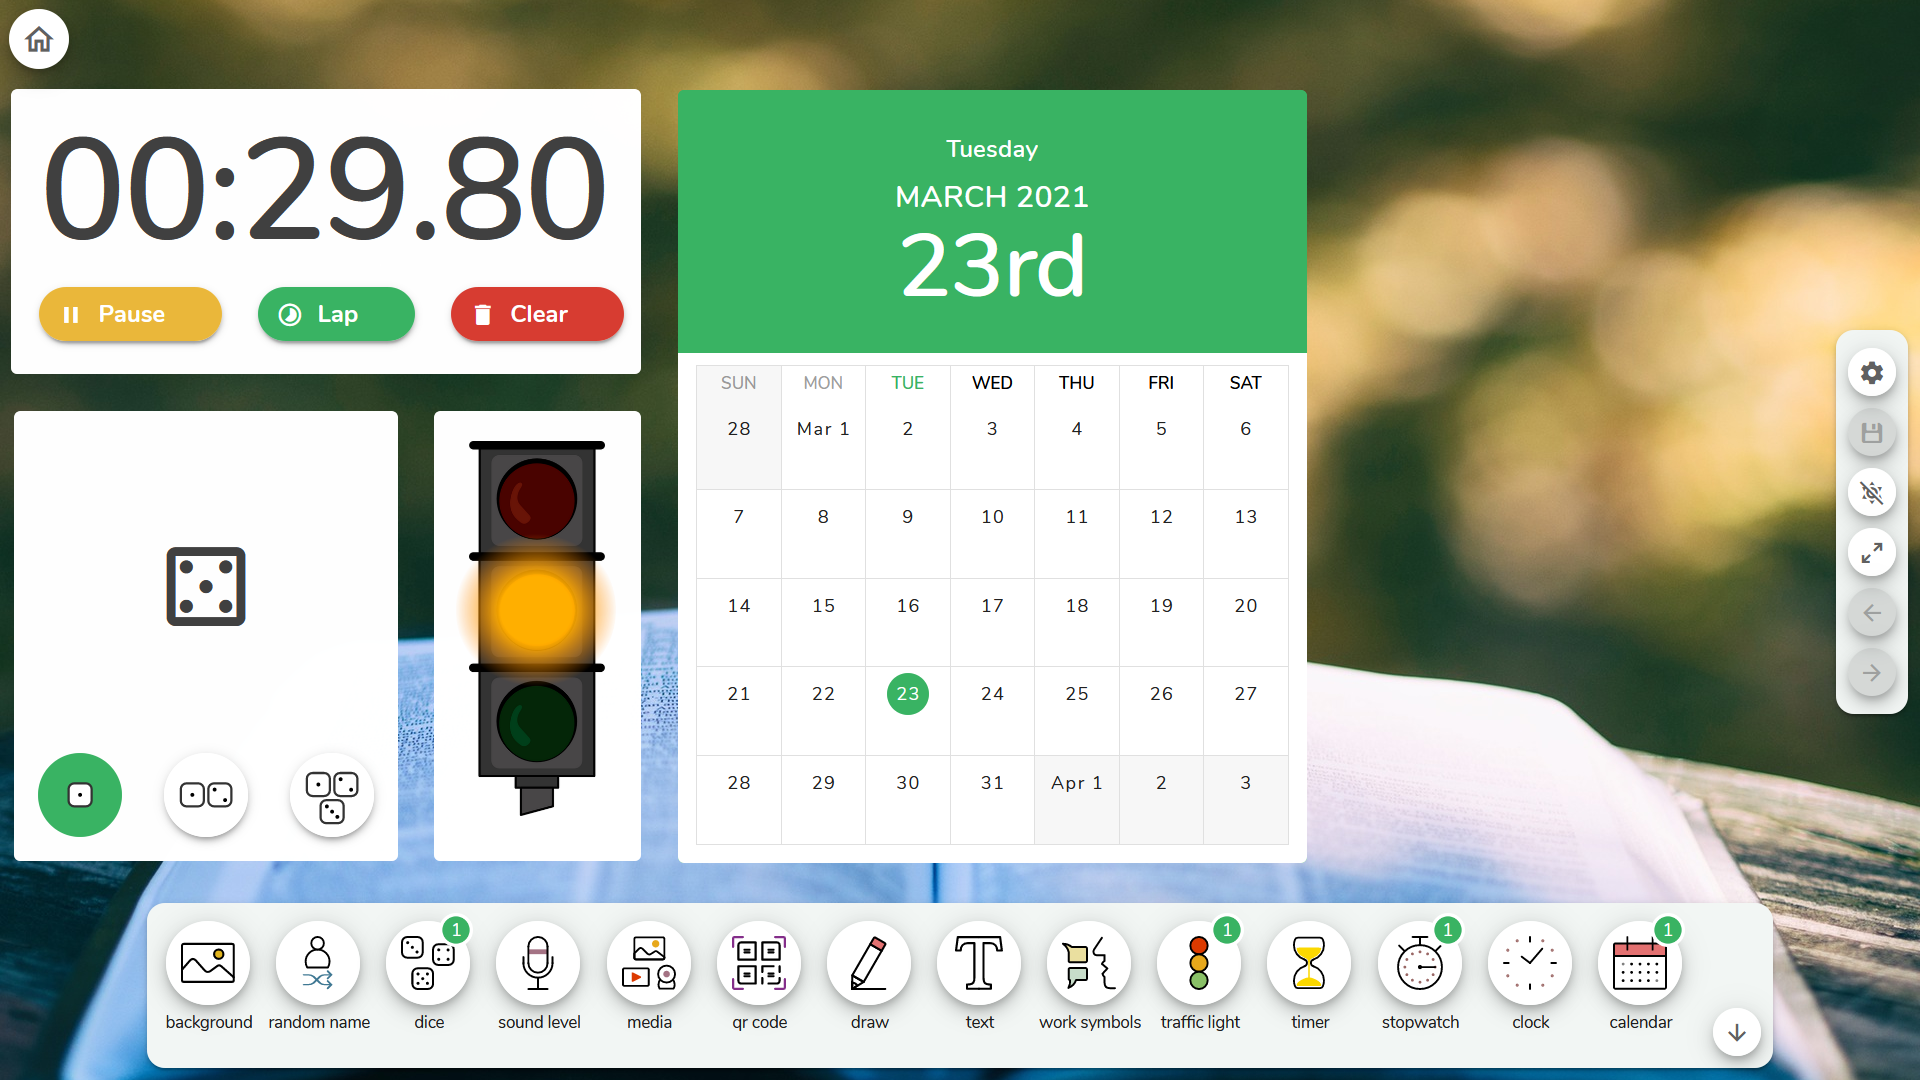
\includegraphics[width=1\textwidth]{Figures/classroomscreen.png}
	\caption{Ukázka webu classroomscreen.com}
	\label{fig:classroomscreen}
\end{figure}



\subsection{Inspirace - whiteboard.fi}
\label{sec:2.3}
Dále byla zanalyzována stránka \underline{whiteboard.fi}.
Tento web registrovaný pod finskou národní doménou je orientovaný především pro využití ve školním prostředí.
Po vytvoření místnosti je zobrazeno plátno o předem dané velikosti, které se ostatním uživatelům během úpravy neaktualizuje.
Pro odeslání aktuálního stavu plátna je potřeba stisknout tlačítko Push.
V rámci místnosti je možné vytvářet více pláten a libovolně mezi nimi přepínat a upravovat je.
Web obsahuje základní nástroje jako kreslení, přidání textu, obrázku či speciální nástroje jako notový zápis a další a jak již bylo zmíněno, jeho využití je tedy především ve škole.
Stránka rovněž využívá Canvas API pro vykreslení grafiky, ale navíc používá protokol WebSocket, díky kterému podporuje spolupráci více uživatelů.

Hlavní inspirací u tohoto webu bylo přepínání hustoty mřížky na pozadí plátna, díky které je možné lépe umístit či vyměřit určité objekty.
\begin{figure}[h!]
	\centering
	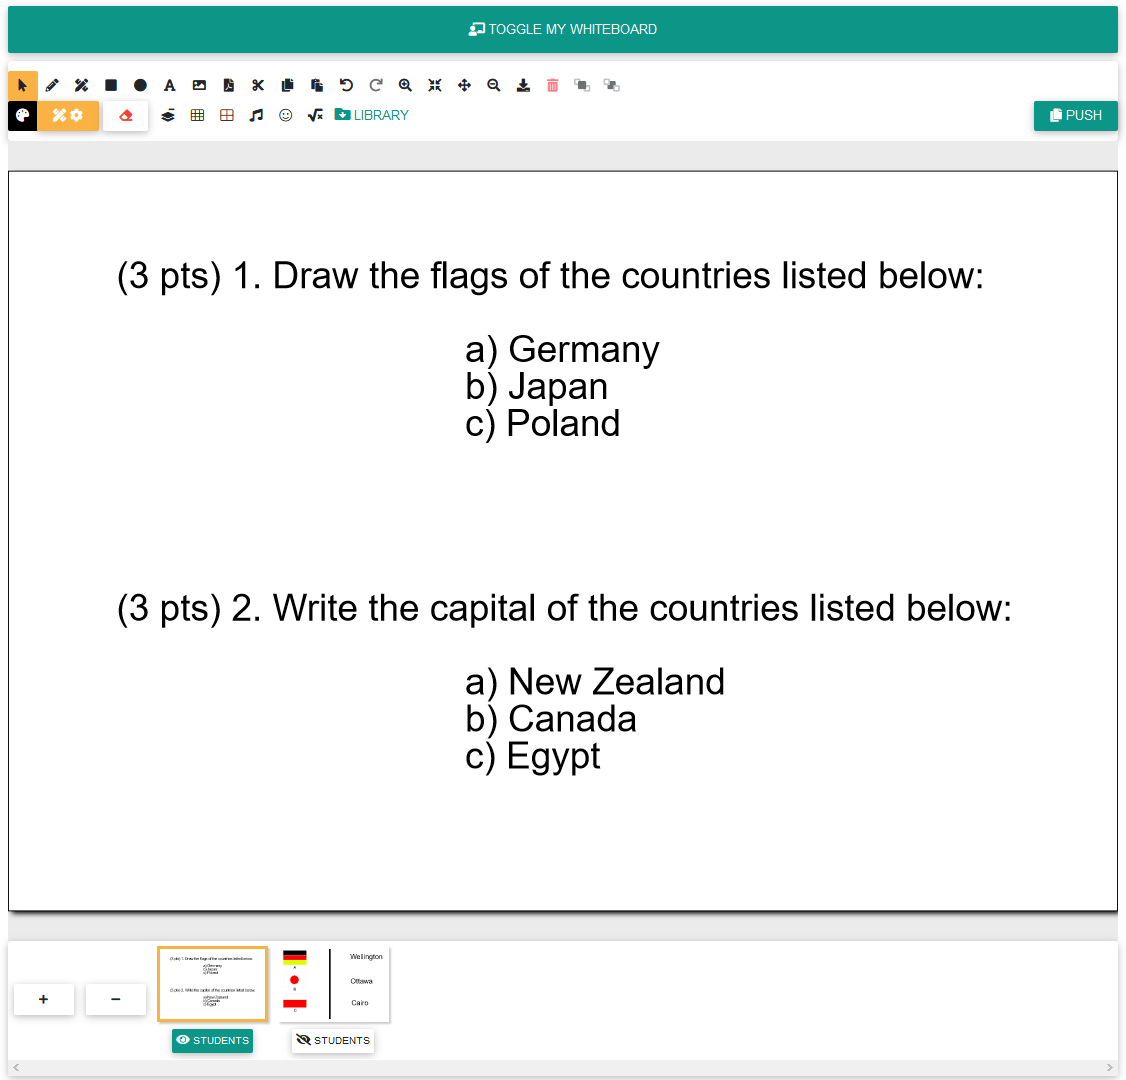
\includegraphics[width=1\textwidth]{Figures/whiteboard.png}
	\caption{Ukázka webu whiteboard.fi}
	\label{fig:whiteboard}
\end{figure}



\subsection{Inspirace - whiteboardfox.com}
\label{sec:2.4}
Třetím webem pro inspiraci byl \underline{whiteboardfox.com}.
Tento web oproti předchozím mnohem více funguje na myšlence virtuální sdílené tabule.

Velikost plátna tabule není omezena velikostí okna prohlížeče a veškeré úpravy tabule jsou automaticky distribuované všem uživatelům.
Inspirace těmito dvěma vlastnostmi jsou ostatně hlavním důvodem, proč je zde tato stránka zmíněna.

Uživatelské rozhraní však nepůsobí příliš moderně, není responzivní a orientace v něm je relativně složitá, jelikož většina nástrojů je schována pod tlačítkem nastavení, což pro mnoho uživatelů nemusí být intuitivní.
Opět se zde objevuje využití Canvasu a také WebSocket, který zmíněný web používá ke sdílení dat a díky čemuž je tento web určen pro spolupráci více uživatelů.



\subsection{Inspirace - collboard.com}
\label{sec:2.5}
Předposledním vybraným řešením virtuální tabule je stránka \underline{collboard.com}.
Tato stránka vylepšuje nedostatky předchozího webu co se týče náročnosti používání uživatelského rozhraní a doplňuje jej o celou řadu možností úprav jednotlivých objektů, jako např. změna tloušťky čáry u kreslení či změna řezu písma u textu a další.
Veškeré objekty lze libovolně vybírat a přesouvat či dále měnit.
Web dále umožňuje přidávat různé pluginy, které využitelnost celého řešení ještě více rozšiřují.
U tabule je možné zadat také její název, což se může zdát jako drobnost, nicméně tento detail může být užitečný pro identifikaci sdílené tabule např. v emailové pozvánce.
Na místě je také tlačítko vrácení na počáteční pozici.
Může se totiž lehce stát, že se uživatel při pohybu po tabuli ztratí.
Použité technologie se oproti předchozímu řešení nijak neliší.

Tento web byl velmi výraznou inspirací pro finální řešení bakalářské práce, jelikož nabízí opravdu moderní, responzivní prostředí, plné užitečných nástrojů a velmi dobře promyšlených řešení případných uživatelských problémů.
Jedná se tak o velmi užitečný nástroj pro sdílení virtuální tabule.



\subsection{Inspirace - miro.com}
\label{sec:2.6}
Nejrozsáhlejší a nejpropracovanější stránkou z výběru je \underline{miro.com}.
Oproti collboard.com je tento web rozšířen o další spoustu nástrojů vhodných pro větší projekty.
Poskytuje vlastní API pro tvorbu pluginů a také integraci s aplikacemi třetích stran jako Microsoft Teams či Google Disk.
Nabízí funkci chatu, seznam poznámek, zobrazuje umístění jednotlivých uživatelů.
Přidávat lze mimo základní nástroje také šablony, tedy např. myšlenkové mapy či vývojové diagramy viz. obrázek \ref{fig:miro} a obsahuje také opravdu detailní konfiguraci jednotlivých objektů.
V rámci technologií kromě Canvasu a WebSocket používá navíc Web worker.
Web worker slouží k rozdělení operací do více vláken, čímž se sníží nároky na hlavní vlákno, které je dle specifikací povinné reagovat na uživatelský vstup. \cite{web:MDN/MainThread}
Touto optimalizací je hlavní vlákno schopno dosáhnout vyššího výkonu, což ve výsledku znamená plynulejší běh celého webu.

Největší inspirací byl vizuální styl uživatelského rozhraní a také způsob sdílení tabule prostřednictvím emailu a rozdělení tabule do různých uživatelských režimů - úpravy a zobrazení.
\begin{sidewaysfigure}[h!]
	\centering
	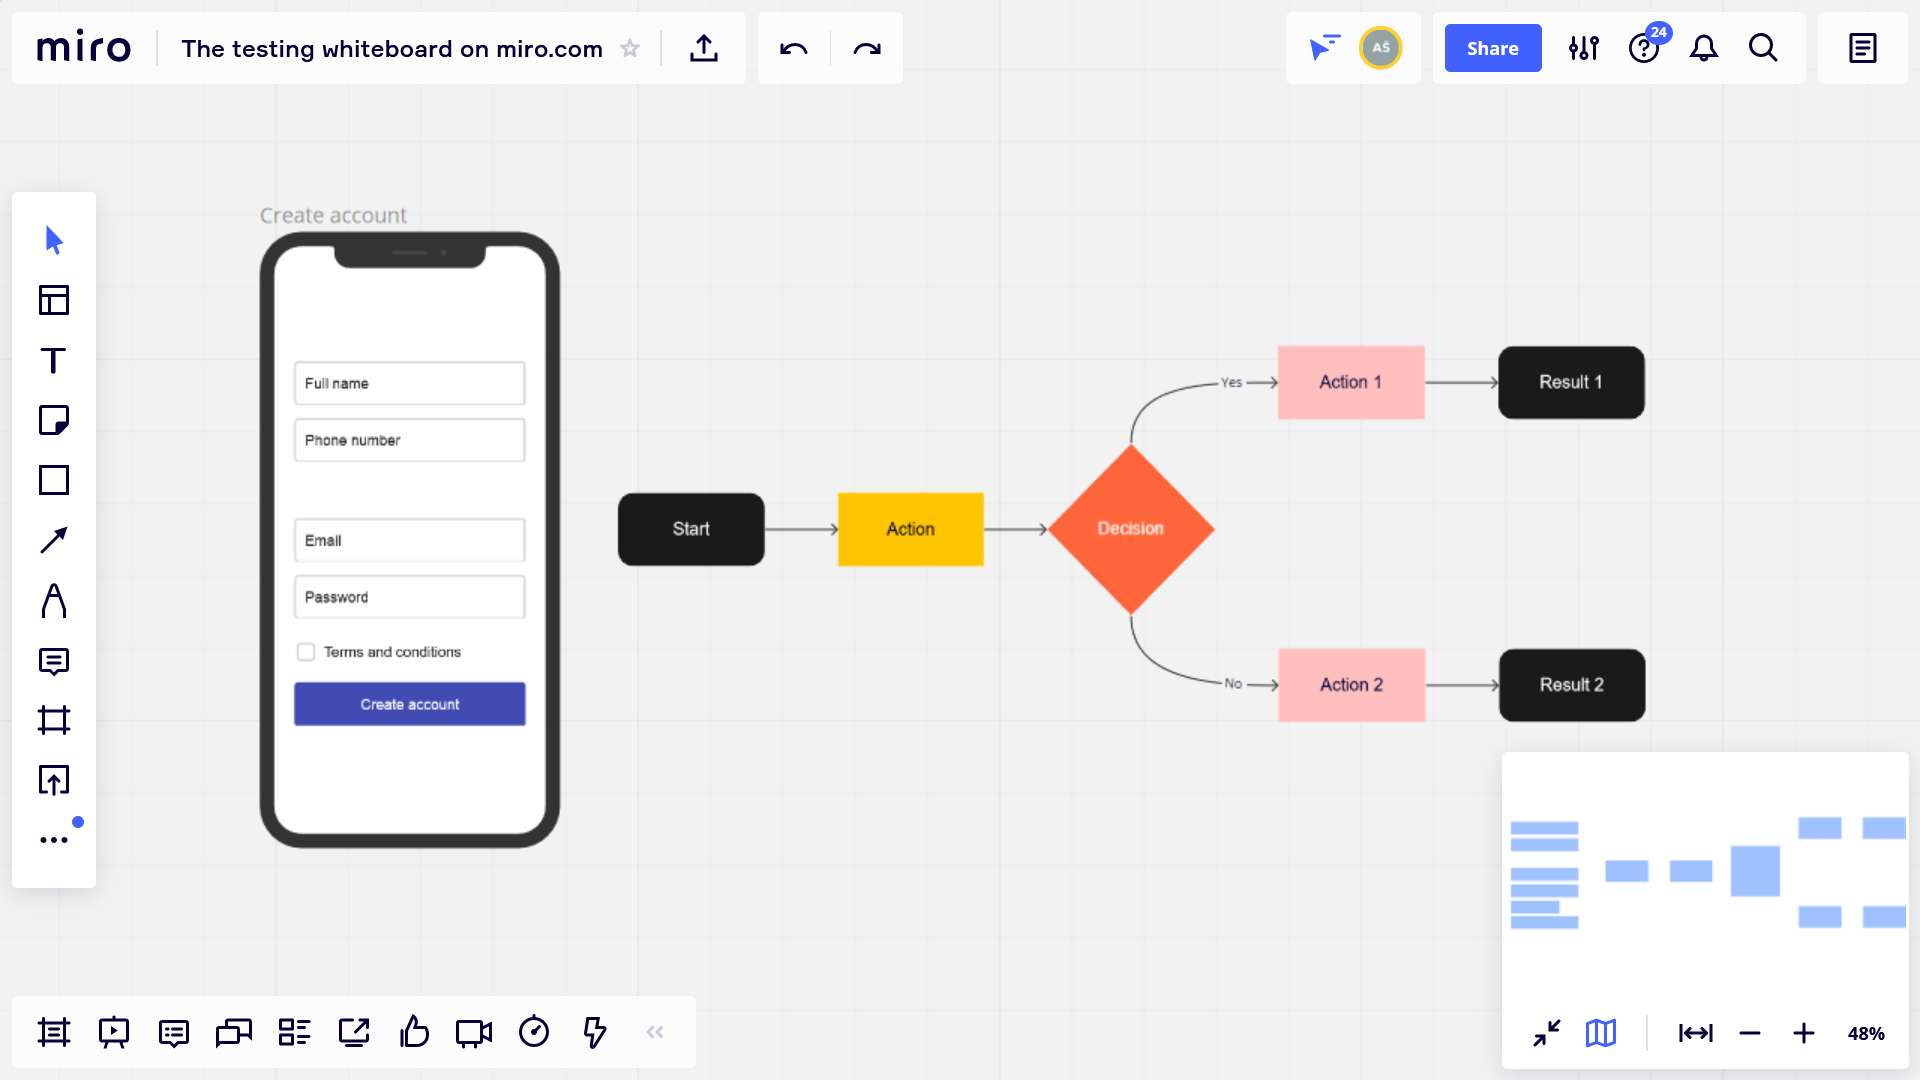
\includegraphics[width=1\textwidth]{Figures/miro.png}
	\caption{Ukázka webu miro.com}
	\label{fig:miro}
\end{sidewaysfigure}
\endinput